\documentclass[border=1mm]{standalone}

\usepackage{amsmath}
\usepackage{xcolor}
\definecolor{den-6}{HTML}{666666}
\usepackage{tkz-tab}
\usetikzlibrary{arrows}

\begin{document}

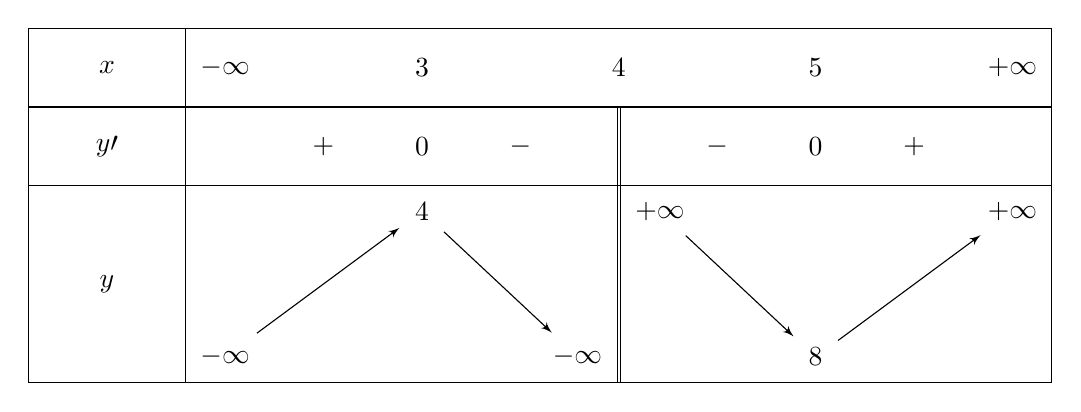
\begin{tikzpicture}
    \tkzTabInit[
        lgt=2, 
        deltacl=.5, 
        espcl=2.5]
        {$x$ / 1, $y\prime$ / 1, $y$ / 2.5}
        {$-\infty$, $3$, $4$, $5$, $+\infty$}%
    \tkzTabLine{ , +, $0$, -, d, -, $0$, +, }
    \tkzTabVar{-/ $-\infty$ / , +/ $4$ /, -D+/ $-\infty$ / $+\infty$ , -/ $8$ /, +/ $+\infty$ /}
    \end{tikzpicture}

\end{document}
